\documentclass[a4paper]{article}
\usepackage[T2A,T1]{fontenc}
\usepackage[utf8]{inputenc}
\usepackage[english, russian]{babel}
\usepackage{graphicx}
\usepackage[hcentering, bindingoffset = 10mm, right = 15 mm, left = 15 mm, top=20mm, bottom = 20 mm]{geometry}
\usepackage{multirow}
\usepackage{lipsum}
\usepackage{amsmath, amstext}
\usepackage{siunitx}
\usepackage{subcaption}
\usepackage{wrapfig}
\usepackage{adjustbox}
\usepackage{enumerate, indentfirst, float}
\usepackage{capt-of, svg}
\usepackage{icomma}

\usepackage[T2A]{fontenc} %кодировка
\usepackage[utf8]{inputenc} %кодировка исходного кода
\usepackage[english,russian]{babel} %локализация и переносы








\newenvironment{bottompar}{\par\vspace*{\fill}}{\clearpage}
 
\begin{document}


\begin{titlepage}
	\centering
	\vspace{5cm}
	{\scshape\LARGE МОСКОВСКИЙ ФИЗИКО-ТЕХНИЧЕСКИЙ ИНСТИТУТ (НАЦИОНАЛЬНЫЙ ИССЛЕДОВАТЕЛЬСКИЙ УНИВЕРСИТЕТ)
 \par}
	\vspace{4cm}
	{\scshape\Large Лабораторная работа №1 \par}
	\vspace{1cm}
	{\huge\bfseries Измерение температуры пламени  \par}
    {\huge\bfseries  методом обращения спектральных линий  \par}
\vspace{1cm}
\begin {figure}[H]
\begin{center}

\includegraphics[width=0.6\textwidth]{faki.png}
\end{center}
\end {figure}
\vspace{1cm}
\begin{flushright}
	{\large выполнили студенты 2 курса группы Б03-104}\par
	\vspace{0.3cm}
	{\LARGE Платонов Никита}\par
    \vspace{0.3cm}
    {\LARGE Алаторцев Кирилл}\par
    \vspace{0.3cm}
    {\LARGE Недопекин Валерий}\par
\end{flushright}
	\vfill
% Bottom of the page
	г. Долгопрудный, 2023 г.
\end{titlepage}


\section*{Аннотация:}
В данной работе производится исследование сопла Лаваля и различных режимов истечения воздуха из него. Для визуализации потока используется теневой и шлирен методы. Измеряются давление газа в ресивере и давление в струе насадком полного напора. По измеренным данным определяются параметры потока на выходе из сопла и сравниваются с рассчитанными по одномерной теории. 

\section*{Цель работы:}
Исследовать режимы истечения газа из двух сопел Лаваля: рассчитать числа Маха для каждого случая двумя способами, определить режим истечения из сопел, найти степени нерасчётности.

\section*{Задачи: }
\begin{numerate} 
  \item -Вывести формулу для числа Маха (физического и геометрического)
  \item -Используя python реализовать итерационный метод расчёта числа Маха
  \item -Изучить режимы работы сопла и получить их изображения на практике
  \item -Рассчитать степени нерасчётности
\end{numerate}

\vspace{4cm}

\begin {figure}[H]
\begin{center}
\large{ВСЕ КОДЫ К РАБОТЕ МОЖНО НАЙТИ ЗДЕСЬ:}
\par

\includegraphics[width=0.3\textwidth]{qr.png}
\end{center}
\end {figure}




\newpage
\section*{Теоретические сведения:}
Сопло - закрытый канал переменного сечения, предназначенный для разгона газа или жидкости. 
\vspace{0.3cm}

Сопло Лавяля - сопло, которое используется для получения сверхзвукового потока за счёт прохода потока газа сначала через сужающийся канал, а затем через расширяющийся.

\par
Будем считать, что течение газа в канале стационарное, одномерное\footnote[1]{параметры потока зависят только от координаты вдоль оси трубы}, адиабатическое, а газ является идеальным и калорически совершенным\footnote[2]{теплоёмкости газа $c_p$ и $c_v$ постоянны}. 
\par
\vspace{0.3cm}
Воспользуемся уравнением неразрывности в дифференциальном виде:

\begin{equation}
    \label{12.1}
    \rho u A = const, 
\end{equation}

где $\rho$ - плотность газа, $u$ - скорость вдоль оси x, $A$ - местное сечение канала. 
\par
\vspace{0.3cm}
Также будем использовать уравнение Эйлера:
\begin{equation}
    \label{12.2}
    u \frac{du}{dx} = - \frac{1}{\rho} \frac{d \rho}{dx}    
\end{equation}



\begin{equation}
    \label{12.3}
    udu= -\frac{1}{\rho}dp = -\frac{dp}{d\rho}\frac{d\rho}{\rho} = -a^2\frac{d\rho}{\rho}
\end{equation}


Произведя логарифмическое дифференцирование ~(\ref{12.1}), можно записать
\begin{equation}
    \label{12.4}
    \frac{d\rho}{\rho} + \frac{du}{u} + \frac{dA}{A} = 0
\end{equation}

Подставляя значение $\frac{d\rho}{\rho}$ из ~(\ref{12.4}) в ~(\ref{12.3}), получим
\begin{equation}
    \label{12.5}
    udu = a^2(\frac{du}{u} + \frac{dA}{A})
\end{equation}
или 
$$(u^2 - a^2)\frac{du}{u} = a^2\frac{dA}{A}$$

Заменяя $M = u/a$, получаем соотношения Гюгонио:
\par
\begin{center}
    \fbox{$(M^2 - 1) \frac{du}{u} = \frac{dA}{A},$}
\end{center}
\par
где $M$ - число Маха. \par
\vspace{0.3cm}

Если $M > 1$ , то течение считается сверхзвуковым. При увеличении площади сечения канала скорость растёт. Это происходит потому, что с увеличением скорости газа плотность его уменьшается, и при малых скоростях, когда сжимаемость незначительна, для увеличения скорости необходимо уменьшать сечение канала, а при $M > 1$ уменьшение плотности не компенсируется ростом скорости, и для ускорения газа сечение канала должно увеличиваться.

В случае $M = 1$ получаем, что $dA = 0$, соответсвующее минимальное сечение называется критическим.

Используя уравнение неразрывности и изоэнтропические соотношения для параметров газа в потоке, можно получить связь между параметрами одномерного газового потока и площадью сечения канала:





Связь давления в форкамере, давления за прямым скачком уплотнения и числа Маха имеет следующий вид:

\begin{equation}
    \label{4.9}
    \pi = \frac{p}{p_0}=(1 + \frac{\gamma - 1}{2}M^2)^{-\frac{\gamma}{\gamma - 1}}
\end{equation}

Расчёт геометрического числа Маха для сопла Лаваля производится итерационным методом по следущей формуле:

\begin{equation}
    M_i = \left( \frac{\gamma + 1}{\gamma-1} \left( \frac{A}{A^*}M_{i-1}\right)^{\frac{2(\gamma - 1)}{\gamma+1}} - \frac{2}{\gamma-1}  \right)^{1/2}, M>1 
\end{equation}


Расчёт числа $M$ по отношению $\frac{ {p_0}^{'} }{p_0}$ на прямом скачке производится итерационным методом по следующей формуле:

\begin{equation}
    {M_i}^2 = \frac{\gamma-1}{2\gamma} + \frac{\gamma+1}{2 \gamma} \left( \frac{ {p_0}^{'} }{p_0} \right)^{1-\gamma} \cdot \left[ \frac{2}{\gamma+1} \left( \frac{1}{ {M_{i-1}}^2 } + \frac{\gamma-1}{2} \right)  \right]^{-\gamma},
\end{equation}

где в качестве начального $M_0$ удобно брать $M_\text{геометрическое}$, но можно взять $M_0 = \infty$ или любое другое $M > 1$. 



\section*{Режимы работы сопла:}

Характер распределения параметров течения газа в сопле зависит от степени нерасчетности струи $\eta$, равной отношению давления на выходе из сопла $p_a$ к давлению окружающей среды $p_n$($\eta = p_a / p_n$ ). 
\par
В зависимости от величины нерасчетности $\eta$ сверхзвуковое сопло может работать в следующих режимах: расчетном, недорасширения и перерасширения (рис.1).
\vspace{0.3cm}


\noindent\begin{minipage}{0.3\textwidth}% adapt widths of minipages to your needs
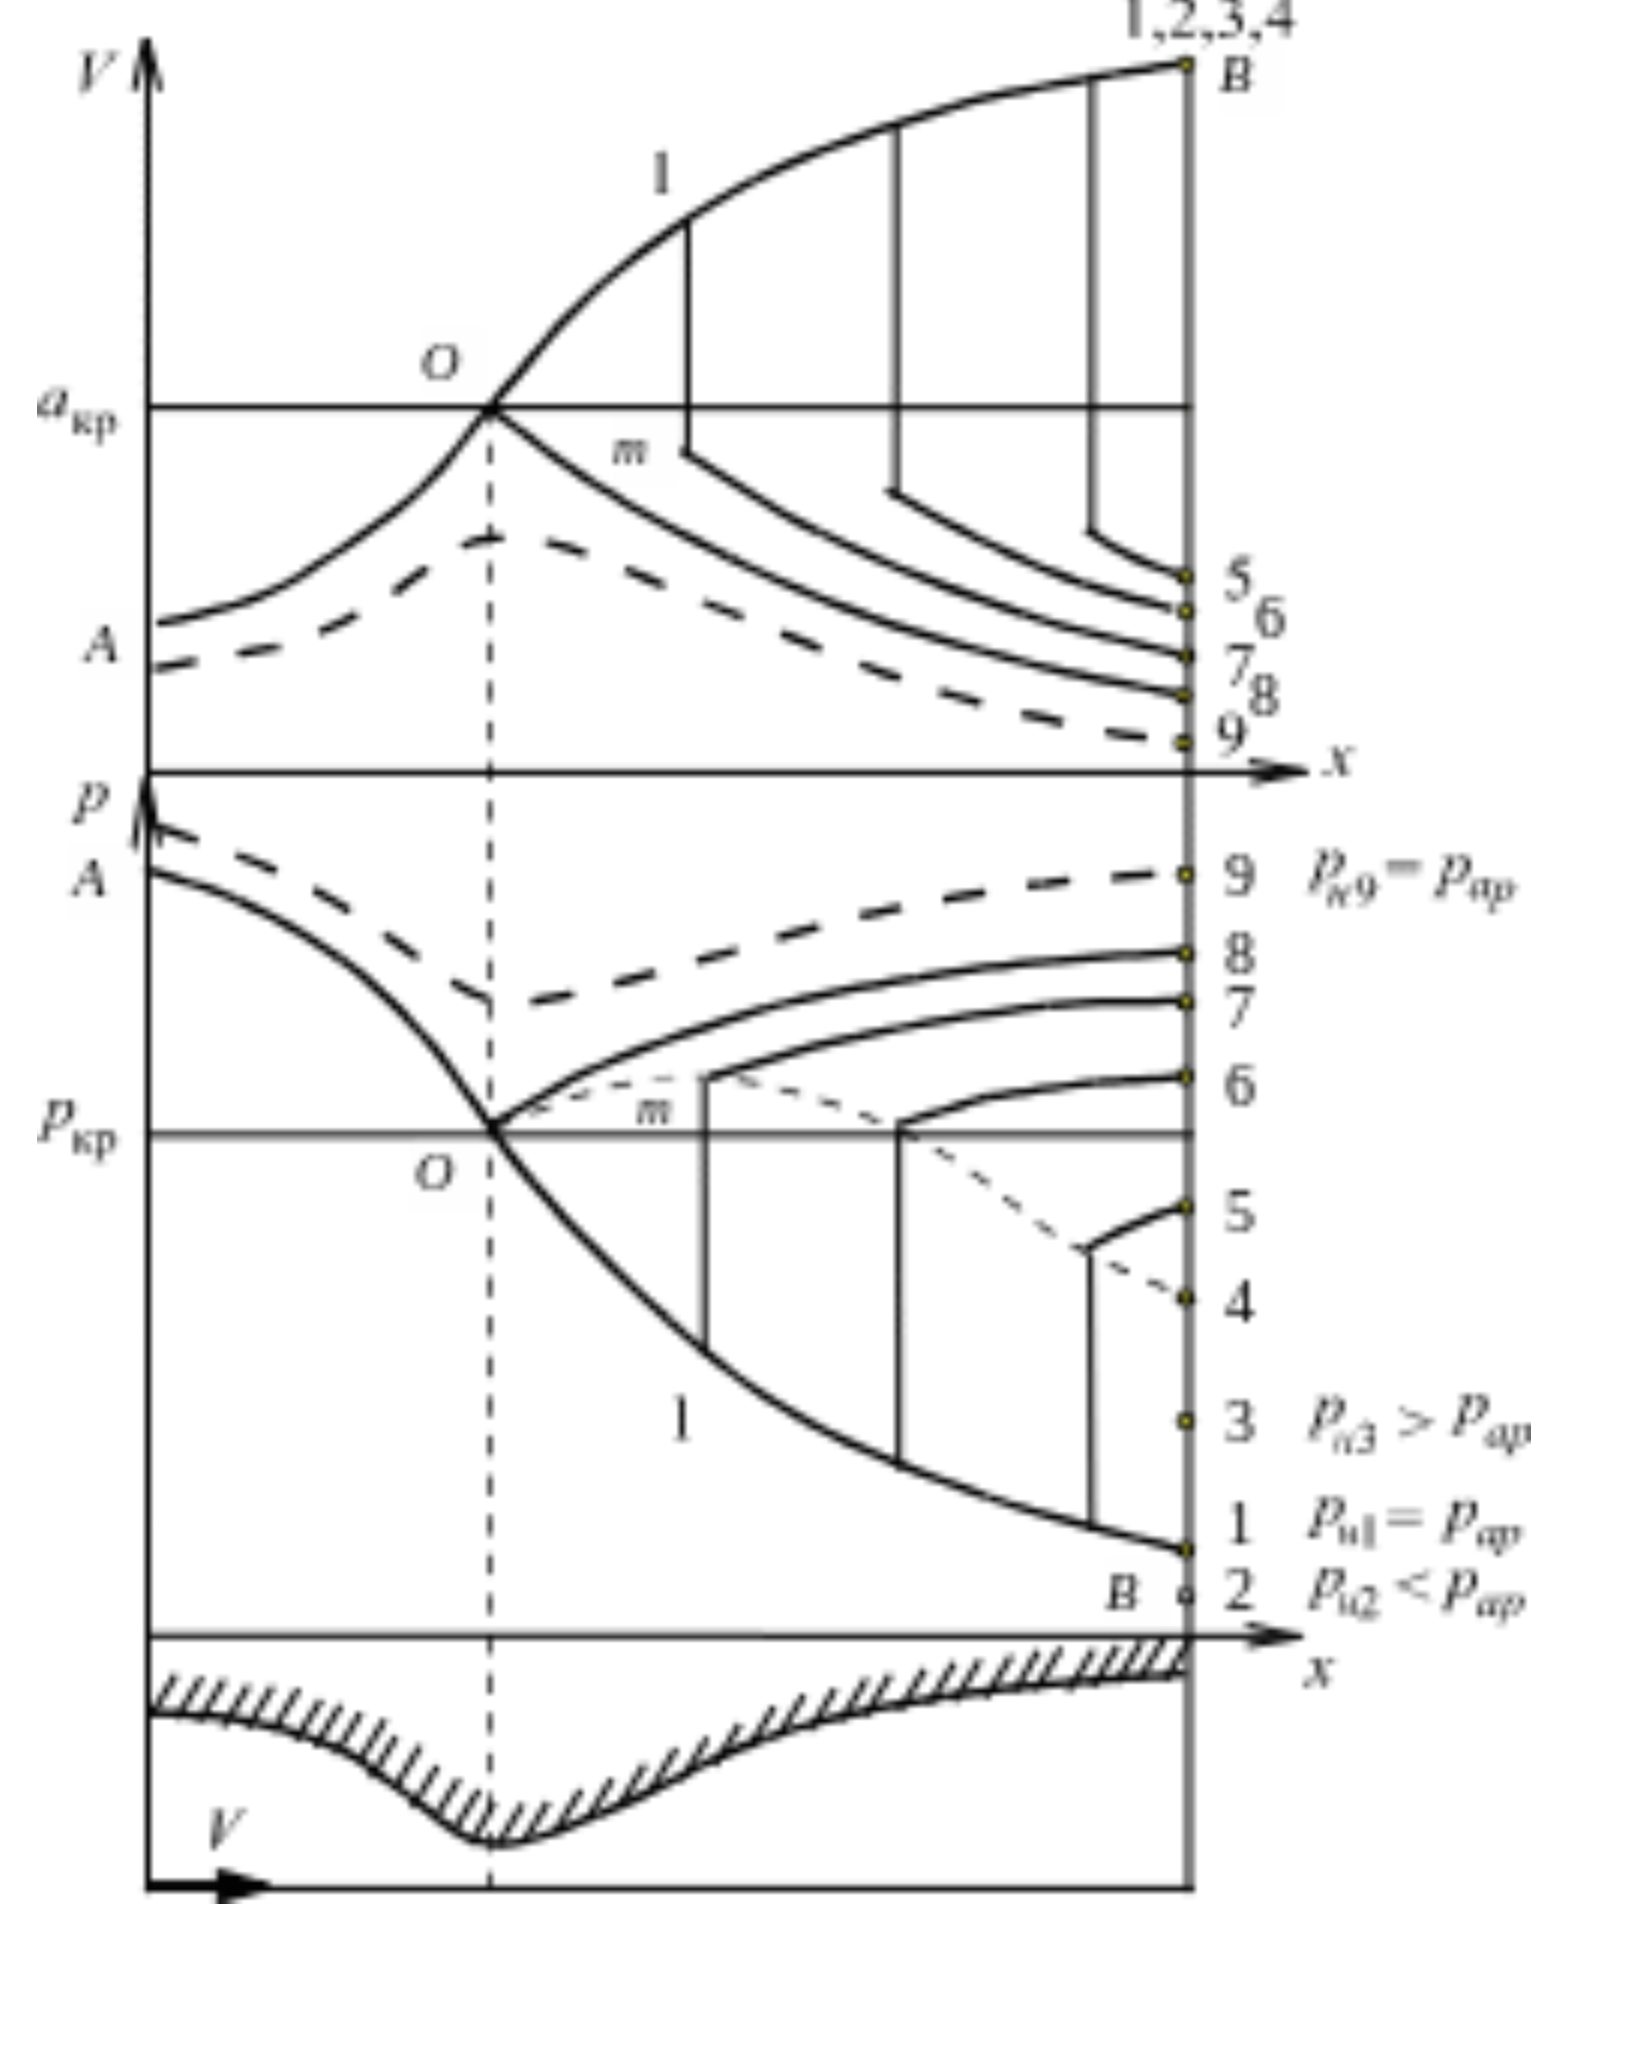
\includegraphics[width=1.35\linewidth]{graph.png} 
\captionof{figure}{\footnotesize{ Распределение давления и скорости в сверхзвуковом потоке при различных режимах работы сопла}}
\end{minipage}%
\hfill%
\begin{minipage}{0.6\textwidth}\raggedright
1. Расчетный режим – давление на срезе сопла равно давлению окружающей среды:$p_a = p_n, \eta = 1$. Изменение скорости и давления газа в сопле изображено линиями АОВ (рис. 1). За соплом сверхзвуковая струя сечением   течет со скоростью при давлении. По мере удаления от сопла скорость газа уменьшается за счет турбулентного смешивания с окружающим газом.
\par
2. Режим недорасширения – давление на срезе сопла больше давления окружающей среды:($\eta > 1$ ). Характер изменения скорости и давления газа в тракте сопла на режиме недорасширения совпадает с расчетным (линия АОВ), давление на срезе сопла и скорость истечения остаются расчетными. Волны пониженного давления из окружающей среды не могут достичь среза сопла – они сносятся сверхзвуковым потоком. Избыточное давление   расходуется на увеличение скорости сверхзвукового потока, но уже за срезом сопла.

\par
3. Режим перерасширения – давление на срезе сопла меньше давления окружающей среды: $p_a < p_n, \eta < 1$  . В таком случае струя начинает сжиматься. При этом возникают косые скачки уплотнения, за которыми давление становится равным $p_a$, а после отражения от оси потока давление возрастает ещё больше $p > p_a$. Далее течение происходит так же, как и в случае с недорасширением.
\end{minipage}










\newpage
\section*{Описание установки:}

Схема установки представлена на Рис. 2. 

\begin {figure}[H]
\begin{center}
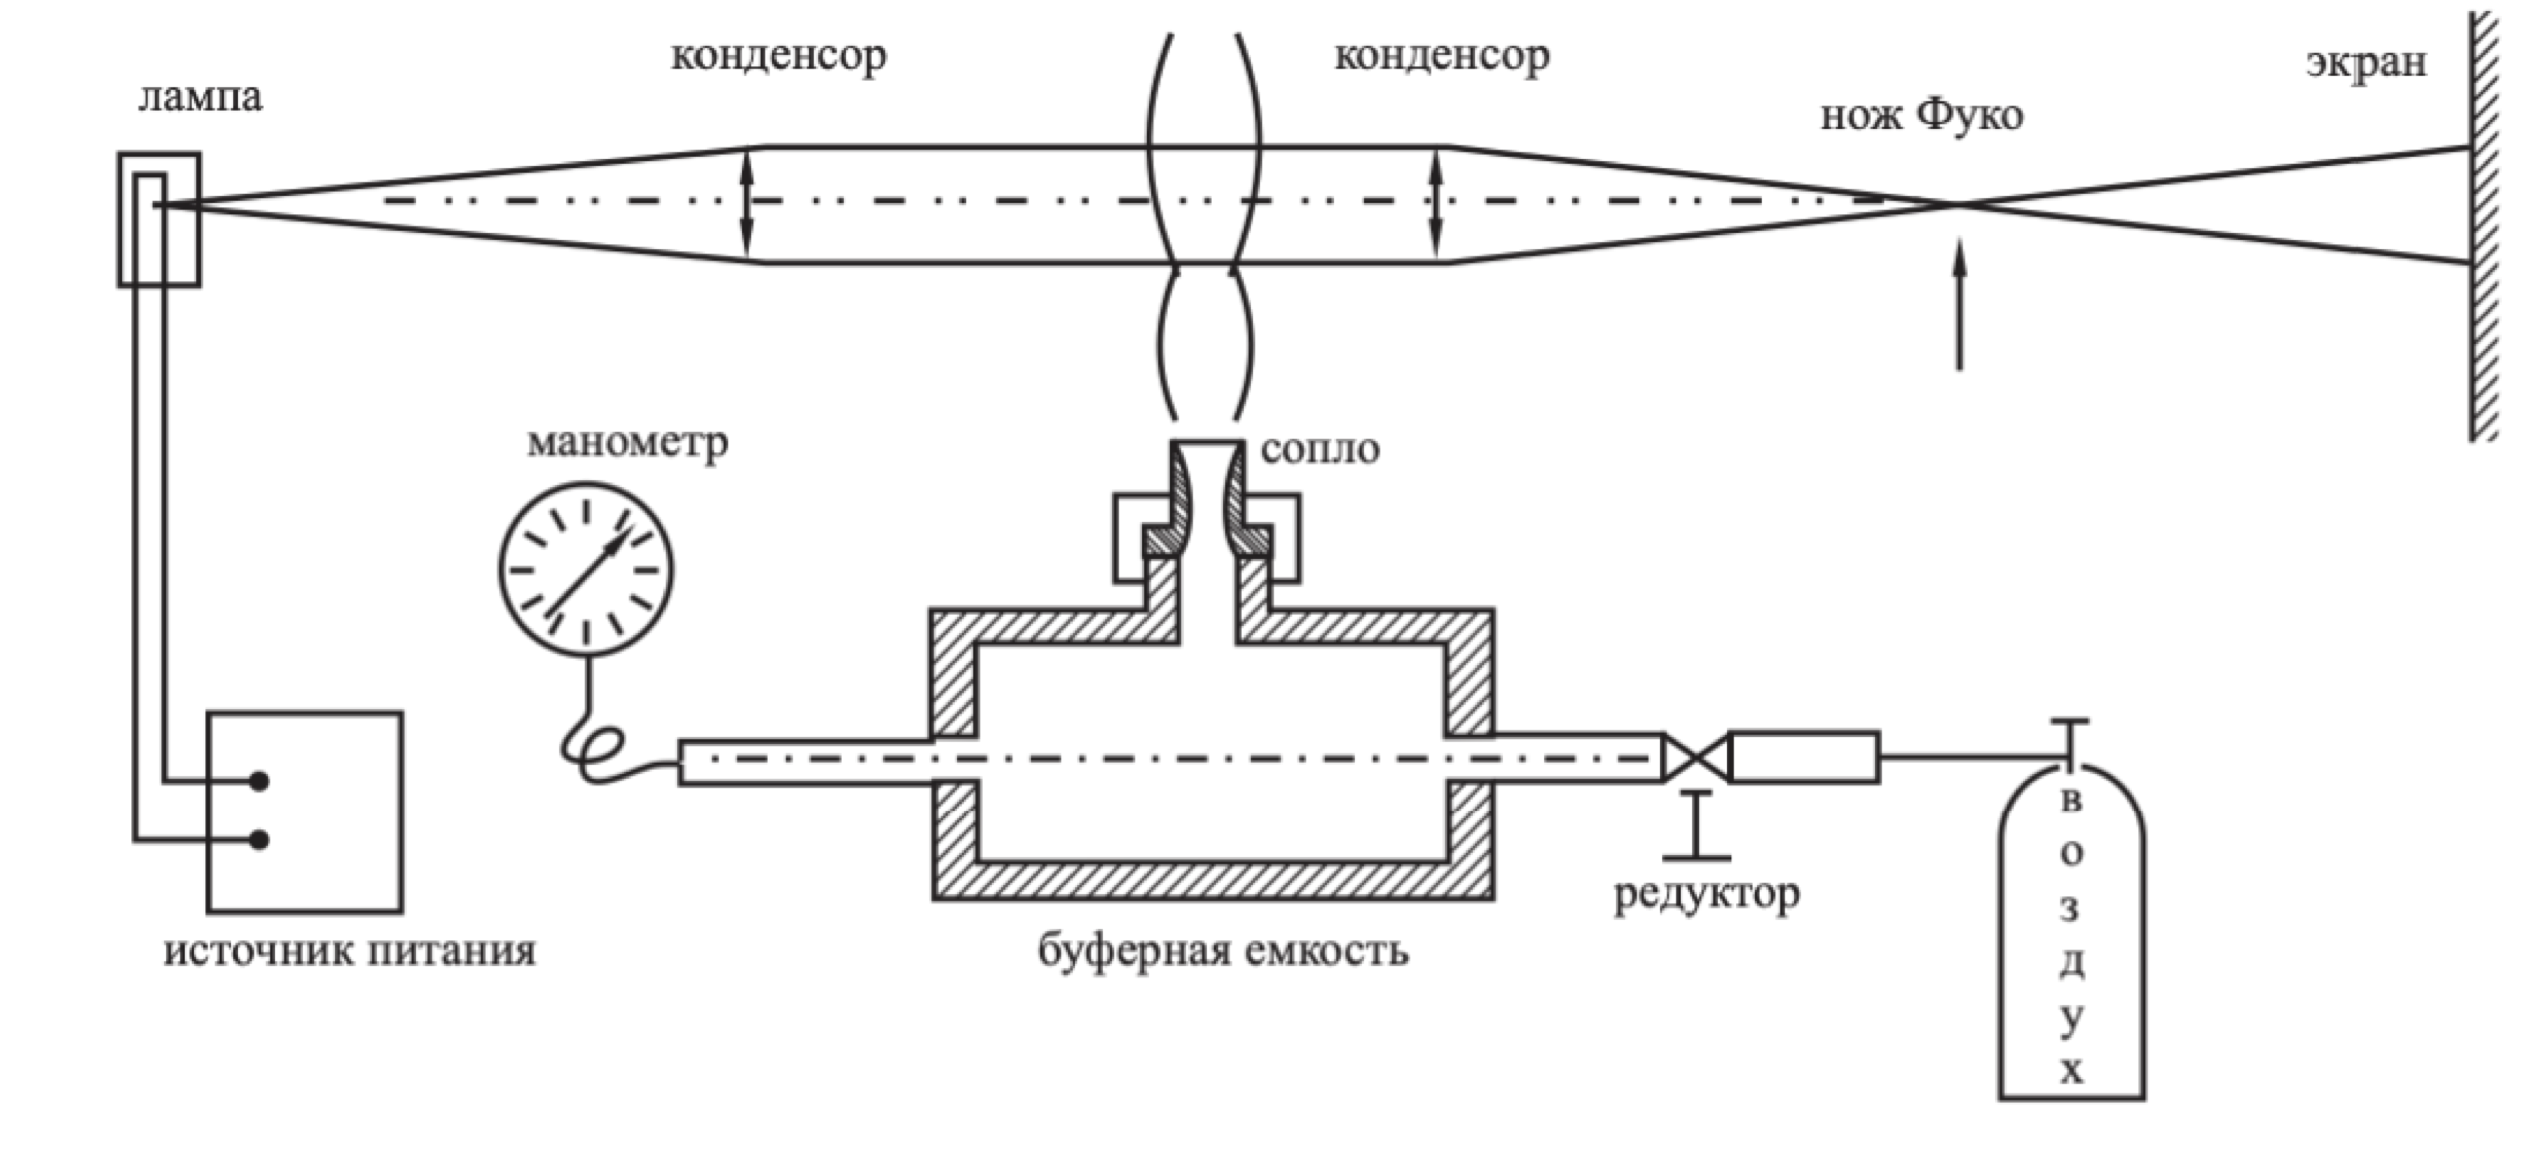
\includegraphics[width=0.9\textwidth]{scheme.png}
\captionof{figure}{Схема установки}
\end{center}
\end {figure}

Воздух из баллона высокого давления через редуктор поступает в ресивер. Ресивер представляет собой толстостенный сосуд объемом 200 см$^3$, служащий для выравнивания параметров газа в предсопловом объёме. Давление в нём устанавливается и регулируется редуктором. К ресиверу подсоединяются сменные сопла (стеклянное или алюминиевое). Установка оснащена визуализирующей оптической системой, которая может быть построена в полутеневом или шлирном варианте. Она состоит из точечного источника света (лампы), набора линз, ножа Фуко и экрана. Давление в ресивере измеряется пружинным манометром. Для измерения распределения полного давления вдоль струи используется насадок полного давления, соединённый пружинным манометром.




\section*{Результаты измерений:}

Критические и выходные диаметры для двух сопл представлены в таблице 1.

\begin{table}[H]
\centering
\begin{tabular}{|c||c|c|}
\hline
Сопло & Стеклянное & Алюминиевое\\ \hline
$d_\text{кр}$, мм	&1,561	&1,580   \\ \hline
$d_\text{вых}$, мм	&1,725	&2,272	 \\ \hline
\end{tabular}
\caption{Геометрические данные сопл}
\end{table}

Используя формулу (7) при помощи программирования на python рассчитываем геометрические числа Маха:

$$M_{\text{стекло}} = 1,563 $$

$$M_{\text{алюминий}} = 2,235 $$

А затем физические при помощи формулы (8), используя для просчёта $M_\text{геометрическое} $в качестве начального:

$$M_{\text{стекло физическое}} = 1,59 $$

$$M_{\text{алюминий физическое}} = 2,3 $$


Также были получены следующие данные (представлены в таблице 2), где $p_0$ - давление в форкамере, а $p_{0}^{'}$ - давление в выходном срезе сопла.


\begin{table}[H]
\centering
\begin{tabular}{|c||c|c|}
\hline
Сопло & Стеклянное & Алюминиевое\\ \hline
$p_{\text{кв.расч}}$, атм	&4,02	&11,23   \\ \hline
$ p_{0}^{'} $, атм	&4,1	&6,235	 \\ \hline
$ p_{\text{недо}} $, атм	&15,9	&17,8	 \\ \hline
$ p_{\text{пере}} $, атм	&3,8	&5,5	 \\ \hline
\end{tabular}
\caption{Начальное давление и за прямым скачком уплотнения квазирасчётного режима и давление в форкамере нерасчётного режима}
\end{table}



Используя формулу (6) для давления окружающей среды $p_0$ = 1 атм, получаем уточнение для давления в форкамере расчётного режима и давление на выходе из сопла, численно равное степени нерасчётности, в силу того, что давление окружающей среды 1 атм.

\begin{table}[H]
\centering
\begin{tabular}{|c||c|c|}
\hline
Сопло & Стеклянное & Алюминиевое\\ \hline
$ p_{\text{расч}} $, атм	&4,27	&11,2	 \\ \hline
$p_\text{вых}$, атм	&0,996	&0,992   \\ \hline
\end{tabular}
\caption{Начальное давление в расчётном режиме и давление на выходе из сопла}
\end{table}

Степени нерасчётности для недорасширения и перерасширения, а также для расчётного режима представлены в таблице 4.


\begin{table}[H]
\centering
\begin{tabular}{|c||c|c|}
\hline
Сопло & Стеклянное & Алюминиевое\\ \hline
$\eta_\text{расч}$ & 0,94 & 1,00 \\ \hline
$\eta_\text{недо}$ & 3,72 & 1,59 \\ \hline
$\eta_\text{пере}$ & 0,89 & 0,49 \\ \hline
\end{tabular}
\caption{Степени нерасчётности для трёх режимов}
\end{table}

Для всех режимов получены изображения, представленные в следующем пункте.


\section*{Иллюстрации:}


\subsection*{Расчётный режим}
\begin{figure}[h]
\begin{minipage}[h]{0.5\linewidth}
\center{\includegraphics[width=0.95\linewidth]{eq_glass.png} \\ а)}
\end{minipage}
\hfill
\begin{minipage}[h]{0.5\linewidth}
\center{\includegraphics[width=0.95\linewidth]{eq_al.png} \\ б)}
\end{minipage}
\caption{Режим, близкий к расчётному (а - стеклянное сопло, б - алюминиевое сопло)}
\label{ris:image1}
\end{figure}

Профиль струи при квазирасчётном режиме почти прямой. Для измерения давлений, использованных для вычисления числа Маха физическим методом, трубка полных напоров перемещается вплотную к срезу сечения сопла
\newpage
\subsection*{Недорасширение}

\begin{figure}[h]
\begin{minipage}[h]{0.5\linewidth}
\center{\includegraphics[width=0.95\linewidth]{nedo_glass.png} \\ а)}
\end{minipage}
\hfill
\begin{minipage}[h]{0.5\linewidth}
\center{\includegraphics[width=0.95\linewidth]{nedo_al.png} \\ б)}
\end{minipage}
\caption{Недорасширение (а - стеклянное сопло, б - алюминиевое сопло)}
\label{ris:image1}
\end{figure}


Видна характерная для недорасширения бочкообразная форма границы струи, связанная с тем, что сразу за срезом сопла начинается расширение струи, так как давление в ней больше, чем в окружающей среде, и происходит перерасширение, и далее сжатие и расширение периодически повторяются до выравнивания скоростей в струе. Похожее происходит в перерасширении, за исключением того, что сначала идет сжатие.

\subsection*{Перерасширение}

\begin{figure}[h]
\begin{minipage}[h]{0.5\linewidth}
\center{\includegraphics[width=0.95\linewidth]{pere_glass.png} \\ а)}
\end{minipage}
\hfill
\begin{minipage}[h]{0.5\linewidth}
\center{\includegraphics[width=0.95\linewidth]{pere_al.png} \\ б)}
\end{minipage}
\caption{Перерасширение (а - стеклянное сопло, б - алюминиевое сопло)}
\label{ris:image1}
\end{figure}







\section*{Вывод:}
В ходе работы были исследованы режимы истечения газа из двух сопел Лаваля, получены числа Маха двумя способами, давшими приблизительно одинаковые результаты; определены режимы течений и посчитаны степени нерасчётности. В условиях, созданных для эксперимента, можно пользоваться одномерной газовой динамикой.




\end{document}